% Created by tikzDevice version 0.12.6 on 2026-07-03 11:54:53
% !TEX encoding = UTF-8 Unicode
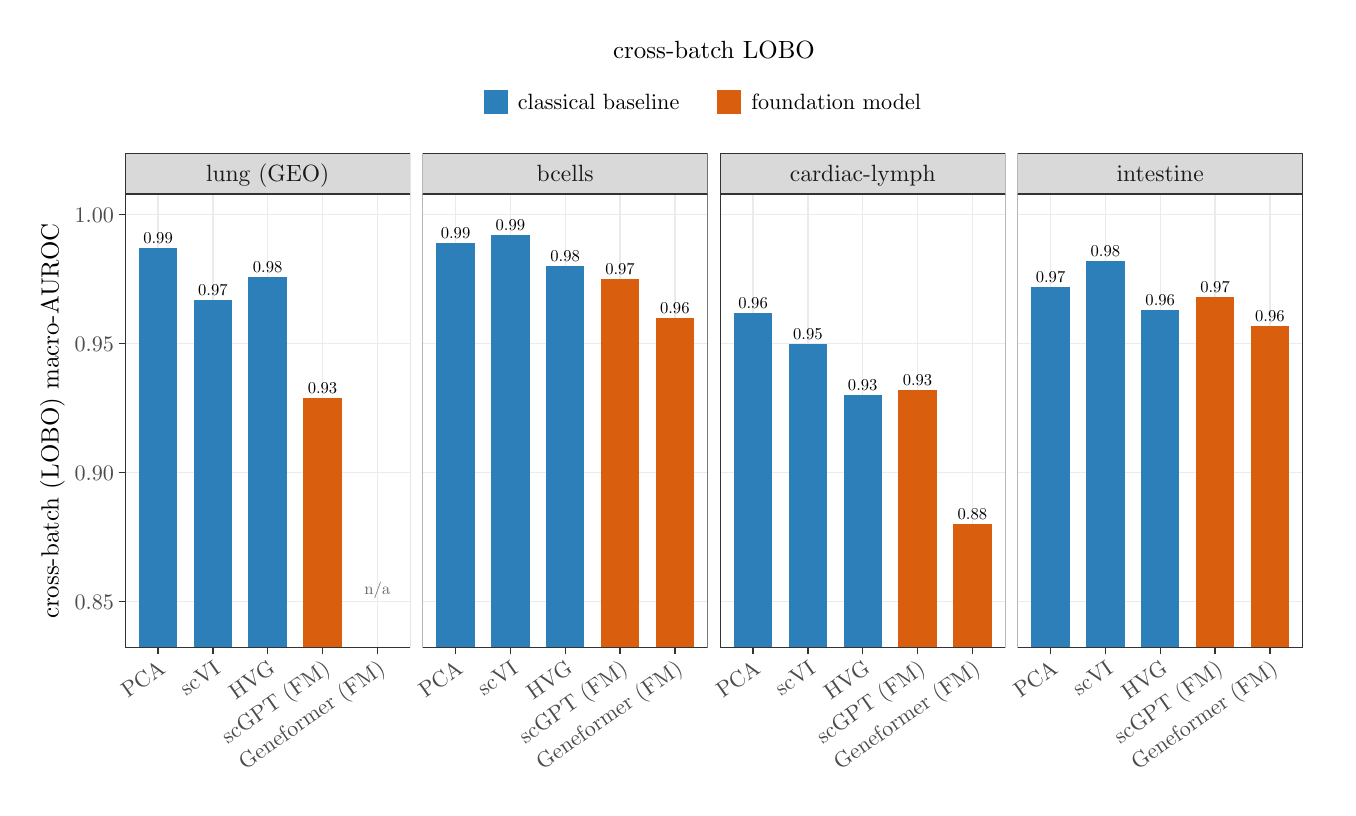
\begin{tikzpicture}[x=1pt,y=1pt]
\definecolor{fillColor}{RGB}{255,255,255}
\path[use as bounding box,fill=fillColor,fill opacity=0.00] (0,0) rectangle (469.75,274.63);
\begin{scope}
\path[clip] (  0.00,  0.00) rectangle (469.75,274.63);
\definecolor{drawColor}{RGB}{255,255,255}
\definecolor{fillColor}{RGB}{255,255,255}

\path[draw=drawColor,line width= 0.5pt,line join=round,line cap=round,fill=fillColor] (  0.00,  0.00) rectangle (469.76,274.63);
\end{scope}
\begin{scope}
\path[clip] ( 35.22, 50.52) rectangle (138.23,214.47);
\definecolor{fillColor}{RGB}{255,255,255}

\path[fill=fillColor] ( 35.22, 50.52) rectangle (138.23,214.47);
\definecolor{drawColor}{gray}{0.92}

\path[draw=drawColor,line width= 0.5pt,line join=round] ( 35.22, 67.29) --
	(138.23, 67.29);

\path[draw=drawColor,line width= 0.5pt,line join=round] ( 35.22,113.86) --
	(138.23,113.86);

\path[draw=drawColor,line width= 0.5pt,line join=round] ( 35.22,160.44) --
	(138.23,160.44);

\path[draw=drawColor,line width= 0.5pt,line join=round] ( 35.22,207.02) --
	(138.23,207.02);

\path[draw=drawColor,line width= 0.5pt,line join=round] ( 47.11, 50.52) --
	( 47.11,214.47);

\path[draw=drawColor,line width= 0.5pt,line join=round] ( 66.92, 50.52) --
	( 66.92,214.47);

\path[draw=drawColor,line width= 0.5pt,line join=round] ( 86.73, 50.52) --
	( 86.73,214.47);

\path[draw=drawColor,line width= 0.5pt,line join=round] (106.54, 50.52) --
	(106.54,214.47);

\path[draw=drawColor,line width= 0.5pt,line join=round] (126.34, 50.52) --
	(126.34,214.47);
\definecolor{fillColor}{RGB}{44,127,184}

\path[fill=fillColor] ( 40.17,-724.50) rectangle ( 54.04,194.91);

\path[fill=fillColor] ( 59.98,-724.50) rectangle ( 73.85,176.28);

\path[fill=fillColor] ( 79.79,-724.50) rectangle ( 93.66,184.66);
\definecolor{fillColor}{RGB}{217,95,14}

\path[fill=fillColor] ( 99.60,-724.50) rectangle (113.47,140.88);
\definecolor{drawColor}{RGB}{0,0,0}

\node[text=drawColor,anchor=base,inner sep=0pt, outer sep=0pt, scale=  0.60] at ( 47.11,196.55) {0.99};

\node[text=drawColor,anchor=base,inner sep=0pt, outer sep=0pt, scale=  0.60] at ( 66.92,177.92) {0.97};

\node[text=drawColor,anchor=base,inner sep=0pt, outer sep=0pt, scale=  0.60] at ( 86.73,186.31) {0.98};

\node[text=drawColor,anchor=base,inner sep=0pt, outer sep=0pt, scale=  0.60] at (106.54,142.52) {0.93};
\definecolor{drawColor}{gray}{0.40}

\node[text=drawColor,anchor=base,inner sep=0pt, outer sep=0pt, scale=  0.60] at (126.34, 69.89) {n/a};
\definecolor{drawColor}{gray}{0.20}

\path[draw=drawColor,line width= 0.5pt,line join=round,line cap=round] ( 35.22, 50.52) rectangle (138.23,214.47);
\end{scope}
\begin{scope}
\path[clip] (142.73, 50.52) rectangle (245.74,214.47);
\definecolor{fillColor}{RGB}{255,255,255}

\path[fill=fillColor] (142.73, 50.52) rectangle (245.74,214.47);
\definecolor{drawColor}{gray}{0.92}

\path[draw=drawColor,line width= 0.5pt,line join=round] (142.73, 67.29) --
	(245.74, 67.29);

\path[draw=drawColor,line width= 0.5pt,line join=round] (142.73,113.86) --
	(245.74,113.86);

\path[draw=drawColor,line width= 0.5pt,line join=round] (142.73,160.44) --
	(245.74,160.44);

\path[draw=drawColor,line width= 0.5pt,line join=round] (142.73,207.02) --
	(245.74,207.02);

\path[draw=drawColor,line width= 0.5pt,line join=round] (154.62, 50.52) --
	(154.62,214.47);

\path[draw=drawColor,line width= 0.5pt,line join=round] (174.43, 50.52) --
	(174.43,214.47);

\path[draw=drawColor,line width= 0.5pt,line join=round] (194.23, 50.52) --
	(194.23,214.47);

\path[draw=drawColor,line width= 0.5pt,line join=round] (214.04, 50.52) --
	(214.04,214.47);

\path[draw=drawColor,line width= 0.5pt,line join=round] (233.85, 50.52) --
	(233.85,214.47);
\definecolor{fillColor}{RGB}{44,127,184}

\path[fill=fillColor] (147.68,-724.50) rectangle (161.55,196.77);

\path[fill=fillColor] (167.49,-724.50) rectangle (181.36,199.56);

\path[fill=fillColor] (187.30,-724.50) rectangle (201.17,188.39);
\definecolor{fillColor}{RGB}{217,95,14}

\path[fill=fillColor] (207.11,-724.50) rectangle (220.98,183.73);

\path[fill=fillColor] (226.92,-724.50) rectangle (240.79,169.76);
\definecolor{drawColor}{RGB}{0,0,0}

\node[text=drawColor,anchor=base,inner sep=0pt, outer sep=0pt, scale=  0.60] at (154.62,198.42) {0.99};

\node[text=drawColor,anchor=base,inner sep=0pt, outer sep=0pt, scale=  0.60] at (174.43,201.21) {0.99};

\node[text=drawColor,anchor=base,inner sep=0pt, outer sep=0pt, scale=  0.60] at (194.23,190.03) {0.98};

\node[text=drawColor,anchor=base,inner sep=0pt, outer sep=0pt, scale=  0.60] at (214.04,185.37) {0.97};

\node[text=drawColor,anchor=base,inner sep=0pt, outer sep=0pt, scale=  0.60] at (233.85,171.40) {0.96};
\definecolor{drawColor}{gray}{0.20}

\path[draw=drawColor,line width= 0.5pt,line join=round,line cap=round] (142.73, 50.52) rectangle (245.74,214.47);
\end{scope}
\begin{scope}
\path[clip] (250.24, 50.52) rectangle (353.25,214.47);
\definecolor{fillColor}{RGB}{255,255,255}

\path[fill=fillColor] (250.24, 50.52) rectangle (353.25,214.47);
\definecolor{drawColor}{gray}{0.92}

\path[draw=drawColor,line width= 0.5pt,line join=round] (250.24, 67.29) --
	(353.25, 67.29);

\path[draw=drawColor,line width= 0.5pt,line join=round] (250.24,113.86) --
	(353.25,113.86);

\path[draw=drawColor,line width= 0.5pt,line join=round] (250.24,160.44) --
	(353.25,160.44);

\path[draw=drawColor,line width= 0.5pt,line join=round] (250.24,207.02) --
	(353.25,207.02);

\path[draw=drawColor,line width= 0.5pt,line join=round] (262.12, 50.52) --
	(262.12,214.47);

\path[draw=drawColor,line width= 0.5pt,line join=round] (281.93, 50.52) --
	(281.93,214.47);

\path[draw=drawColor,line width= 0.5pt,line join=round] (301.74, 50.52) --
	(301.74,214.47);

\path[draw=drawColor,line width= 0.5pt,line join=round] (321.55, 50.52) --
	(321.55,214.47);

\path[draw=drawColor,line width= 0.5pt,line join=round] (341.36, 50.52) --
	(341.36,214.47);
\definecolor{fillColor}{RGB}{44,127,184}

\path[fill=fillColor] (255.19,-724.50) rectangle (269.06,171.62);

\path[fill=fillColor] (275.00,-724.50) rectangle (288.87,160.44);

\path[fill=fillColor] (294.81,-724.50) rectangle (308.68,141.81);
\definecolor{fillColor}{RGB}{217,95,14}

\path[fill=fillColor] (314.62,-724.50) rectangle (328.49,143.67);

\path[fill=fillColor] (334.43,-724.50) rectangle (348.29, 95.23);
\definecolor{drawColor}{RGB}{0,0,0}

\node[text=drawColor,anchor=base,inner sep=0pt, outer sep=0pt, scale=  0.60] at (262.12,173.26) {0.96};

\node[text=drawColor,anchor=base,inner sep=0pt, outer sep=0pt, scale=  0.60] at (281.93,162.09) {0.95};

\node[text=drawColor,anchor=base,inner sep=0pt, outer sep=0pt, scale=  0.60] at (301.74,143.46) {0.93};

\node[text=drawColor,anchor=base,inner sep=0pt, outer sep=0pt, scale=  0.60] at (321.55,145.32) {0.93};

\node[text=drawColor,anchor=base,inner sep=0pt, outer sep=0pt, scale=  0.60] at (341.36, 96.88) {0.88};
\definecolor{drawColor}{gray}{0.20}

\path[draw=drawColor,line width= 0.5pt,line join=round,line cap=round] (250.24, 50.52) rectangle (353.25,214.47);
\end{scope}
\begin{scope}
\path[clip] (357.75, 50.52) rectangle (460.75,214.47);
\definecolor{fillColor}{RGB}{255,255,255}

\path[fill=fillColor] (357.75, 50.52) rectangle (460.76,214.47);
\definecolor{drawColor}{gray}{0.92}

\path[draw=drawColor,line width= 0.5pt,line join=round] (357.75, 67.29) --
	(460.75, 67.29);

\path[draw=drawColor,line width= 0.5pt,line join=round] (357.75,113.86) --
	(460.75,113.86);

\path[draw=drawColor,line width= 0.5pt,line join=round] (357.75,160.44) --
	(460.75,160.44);

\path[draw=drawColor,line width= 0.5pt,line join=round] (357.75,207.02) --
	(460.75,207.02);

\path[draw=drawColor,line width= 0.5pt,line join=round] (369.63, 50.52) --
	(369.63,214.47);

\path[draw=drawColor,line width= 0.5pt,line join=round] (389.44, 50.52) --
	(389.44,214.47);

\path[draw=drawColor,line width= 0.5pt,line join=round] (409.25, 50.52) --
	(409.25,214.47);

\path[draw=drawColor,line width= 0.5pt,line join=round] (429.06, 50.52) --
	(429.06,214.47);

\path[draw=drawColor,line width= 0.5pt,line join=round] (448.87, 50.52) --
	(448.87,214.47);
\definecolor{fillColor}{RGB}{44,127,184}

\path[fill=fillColor] (362.70,-724.50) rectangle (376.57,180.93);

\path[fill=fillColor] (382.51,-724.50) rectangle (396.37,190.25);

\path[fill=fillColor] (402.32,-724.50) rectangle (416.18,172.55);
\definecolor{fillColor}{RGB}{217,95,14}

\path[fill=fillColor] (422.13,-724.50) rectangle (435.99,177.21);

\path[fill=fillColor] (441.94,-724.50) rectangle (455.80,166.96);
\definecolor{drawColor}{RGB}{0,0,0}

\node[text=drawColor,anchor=base,inner sep=0pt, outer sep=0pt, scale=  0.60] at (369.63,182.58) {0.97};

\node[text=drawColor,anchor=base,inner sep=0pt, outer sep=0pt, scale=  0.60] at (389.44,191.90) {0.98};

\node[text=drawColor,anchor=base,inner sep=0pt, outer sep=0pt, scale=  0.60] at (409.25,174.20) {0.96};

\node[text=drawColor,anchor=base,inner sep=0pt, outer sep=0pt, scale=  0.60] at (429.06,178.85) {0.97};

\node[text=drawColor,anchor=base,inner sep=0pt, outer sep=0pt, scale=  0.60] at (448.87,168.61) {0.96};
\definecolor{drawColor}{gray}{0.20}

\path[draw=drawColor,line width= 0.5pt,line join=round,line cap=round] (357.75, 50.52) rectangle (460.76,214.47);
\end{scope}
\begin{scope}
\path[clip] ( 35.22,214.47) rectangle (138.23,229.18);
\definecolor{drawColor}{gray}{0.20}
\definecolor{fillColor}{gray}{0.85}

\path[draw=drawColor,line width= 0.5pt,line join=round,line cap=round,fill=fillColor] ( 35.22,214.47) rectangle (138.23,229.18);
\definecolor{drawColor}{gray}{0.10}

\node[text=drawColor,anchor=base,inner sep=0pt, outer sep=0pt, scale=  0.85] at ( 86.73,218.89) {lung (GEO)};
\end{scope}
\begin{scope}
\path[clip] (142.73,214.47) rectangle (245.74,229.18);
\definecolor{drawColor}{gray}{0.20}
\definecolor{fillColor}{gray}{0.85}

\path[draw=drawColor,line width= 0.5pt,line join=round,line cap=round,fill=fillColor] (142.73,214.47) rectangle (245.74,229.18);
\definecolor{drawColor}{gray}{0.10}

\node[text=drawColor,anchor=base,inner sep=0pt, outer sep=0pt, scale=  0.85] at (194.23,218.89) {bcells};
\end{scope}
\begin{scope}
\path[clip] (250.24,214.47) rectangle (353.25,229.18);
\definecolor{drawColor}{gray}{0.20}
\definecolor{fillColor}{gray}{0.85}

\path[draw=drawColor,line width= 0.5pt,line join=round,line cap=round,fill=fillColor] (250.24,214.47) rectangle (353.25,229.18);
\definecolor{drawColor}{gray}{0.10}

\node[text=drawColor,anchor=base,inner sep=0pt, outer sep=0pt, scale=  0.85] at (301.74,218.89) {cardiac-lymph};
\end{scope}
\begin{scope}
\path[clip] (357.75,214.47) rectangle (460.75,229.18);
\definecolor{drawColor}{gray}{0.20}
\definecolor{fillColor}{gray}{0.85}

\path[draw=drawColor,line width= 0.5pt,line join=round,line cap=round,fill=fillColor] (357.75,214.47) rectangle (460.76,229.18);
\definecolor{drawColor}{gray}{0.10}

\node[text=drawColor,anchor=base,inner sep=0pt, outer sep=0pt, scale=  0.85] at (409.25,218.89) {intestine};
\end{scope}
\begin{scope}
\path[clip] (  0.00,  0.00) rectangle (469.75,274.63);
\definecolor{drawColor}{gray}{0.20}

\path[draw=drawColor,line width= 0.5pt,line join=round] ( 47.11, 48.27) --
	( 47.11, 50.52);

\path[draw=drawColor,line width= 0.5pt,line join=round] ( 66.92, 48.27) --
	( 66.92, 50.52);

\path[draw=drawColor,line width= 0.5pt,line join=round] ( 86.73, 48.27) --
	( 86.73, 50.52);

\path[draw=drawColor,line width= 0.5pt,line join=round] (106.54, 48.27) --
	(106.54, 50.52);

\path[draw=drawColor,line width= 0.5pt,line join=round] (126.34, 48.27) --
	(126.34, 50.52);
\end{scope}
\begin{scope}
\path[clip] (  0.00,  0.00) rectangle (469.75,274.63);
\definecolor{drawColor}{gray}{0.30}

\node[text=drawColor,rotate= 35.00,anchor=base east,inner sep=0pt, outer sep=0pt, scale=  0.80] at ( 50.27, 41.96) {PCA};

\node[text=drawColor,rotate= 35.00,anchor=base east,inner sep=0pt, outer sep=0pt, scale=  0.80] at ( 70.08, 41.96) {scVI};

\node[text=drawColor,rotate= 35.00,anchor=base east,inner sep=0pt, outer sep=0pt, scale=  0.80] at ( 89.89, 41.96) {HVG};

\node[text=drawColor,rotate= 35.00,anchor=base east,inner sep=0pt, outer sep=0pt, scale=  0.80] at (109.70, 41.96) {scGPT (FM)};

\node[text=drawColor,rotate= 35.00,anchor=base east,inner sep=0pt, outer sep=0pt, scale=  0.80] at (129.51, 41.96) {Geneformer (FM)};
\end{scope}
\begin{scope}
\path[clip] (  0.00,  0.00) rectangle (469.75,274.63);
\definecolor{drawColor}{gray}{0.20}

\path[draw=drawColor,line width= 0.5pt,line join=round] (154.62, 48.27) --
	(154.62, 50.52);

\path[draw=drawColor,line width= 0.5pt,line join=round] (174.43, 48.27) --
	(174.43, 50.52);

\path[draw=drawColor,line width= 0.5pt,line join=round] (194.23, 48.27) --
	(194.23, 50.52);

\path[draw=drawColor,line width= 0.5pt,line join=round] (214.04, 48.27) --
	(214.04, 50.52);

\path[draw=drawColor,line width= 0.5pt,line join=round] (233.85, 48.27) --
	(233.85, 50.52);
\end{scope}
\begin{scope}
\path[clip] (  0.00,  0.00) rectangle (469.75,274.63);
\definecolor{drawColor}{gray}{0.30}

\node[text=drawColor,rotate= 35.00,anchor=base east,inner sep=0pt, outer sep=0pt, scale=  0.80] at (157.78, 41.96) {PCA};

\node[text=drawColor,rotate= 35.00,anchor=base east,inner sep=0pt, outer sep=0pt, scale=  0.80] at (177.59, 41.96) {scVI};

\node[text=drawColor,rotate= 35.00,anchor=base east,inner sep=0pt, outer sep=0pt, scale=  0.80] at (197.40, 41.96) {HVG};

\node[text=drawColor,rotate= 35.00,anchor=base east,inner sep=0pt, outer sep=0pt, scale=  0.80] at (217.20, 41.96) {scGPT (FM)};

\node[text=drawColor,rotate= 35.00,anchor=base east,inner sep=0pt, outer sep=0pt, scale=  0.80] at (237.01, 41.96) {Geneformer (FM)};
\end{scope}
\begin{scope}
\path[clip] (  0.00,  0.00) rectangle (469.75,274.63);
\definecolor{drawColor}{gray}{0.20}

\path[draw=drawColor,line width= 0.5pt,line join=round] (262.12, 48.27) --
	(262.12, 50.52);

\path[draw=drawColor,line width= 0.5pt,line join=round] (281.93, 48.27) --
	(281.93, 50.52);

\path[draw=drawColor,line width= 0.5pt,line join=round] (301.74, 48.27) --
	(301.74, 50.52);

\path[draw=drawColor,line width= 0.5pt,line join=round] (321.55, 48.27) --
	(321.55, 50.52);

\path[draw=drawColor,line width= 0.5pt,line join=round] (341.36, 48.27) --
	(341.36, 50.52);
\end{scope}
\begin{scope}
\path[clip] (  0.00,  0.00) rectangle (469.75,274.63);
\definecolor{drawColor}{gray}{0.30}

\node[text=drawColor,rotate= 35.00,anchor=base east,inner sep=0pt, outer sep=0pt, scale=  0.80] at (265.29, 41.96) {PCA};

\node[text=drawColor,rotate= 35.00,anchor=base east,inner sep=0pt, outer sep=0pt, scale=  0.80] at (285.09, 41.96) {scVI};

\node[text=drawColor,rotate= 35.00,anchor=base east,inner sep=0pt, outer sep=0pt, scale=  0.80] at (304.90, 41.96) {HVG};

\node[text=drawColor,rotate= 35.00,anchor=base east,inner sep=0pt, outer sep=0pt, scale=  0.80] at (324.71, 41.96) {scGPT (FM)};

\node[text=drawColor,rotate= 35.00,anchor=base east,inner sep=0pt, outer sep=0pt, scale=  0.80] at (344.52, 41.96) {Geneformer (FM)};
\end{scope}
\begin{scope}
\path[clip] (  0.00,  0.00) rectangle (469.75,274.63);
\definecolor{drawColor}{gray}{0.20}

\path[draw=drawColor,line width= 0.5pt,line join=round] (369.63, 48.27) --
	(369.63, 50.52);

\path[draw=drawColor,line width= 0.5pt,line join=round] (389.44, 48.27) --
	(389.44, 50.52);

\path[draw=drawColor,line width= 0.5pt,line join=round] (409.25, 48.27) --
	(409.25, 50.52);

\path[draw=drawColor,line width= 0.5pt,line join=round] (429.06, 48.27) --
	(429.06, 50.52);

\path[draw=drawColor,line width= 0.5pt,line join=round] (448.87, 48.27) --
	(448.87, 50.52);
\end{scope}
\begin{scope}
\path[clip] (  0.00,  0.00) rectangle (469.75,274.63);
\definecolor{drawColor}{gray}{0.30}

\node[text=drawColor,rotate= 35.00,anchor=base east,inner sep=0pt, outer sep=0pt, scale=  0.80] at (372.79, 41.96) {PCA};

\node[text=drawColor,rotate= 35.00,anchor=base east,inner sep=0pt, outer sep=0pt, scale=  0.80] at (392.60, 41.96) {scVI};

\node[text=drawColor,rotate= 35.00,anchor=base east,inner sep=0pt, outer sep=0pt, scale=  0.80] at (412.41, 41.96) {HVG};

\node[text=drawColor,rotate= 35.00,anchor=base east,inner sep=0pt, outer sep=0pt, scale=  0.80] at (432.22, 41.96) {scGPT (FM)};

\node[text=drawColor,rotate= 35.00,anchor=base east,inner sep=0pt, outer sep=0pt, scale=  0.80] at (452.03, 41.96) {Geneformer (FM)};
\end{scope}
\begin{scope}
\path[clip] (  0.00,  0.00) rectangle (469.75,274.63);
\definecolor{drawColor}{gray}{0.30}

\node[text=drawColor,anchor=base east,inner sep=0pt, outer sep=0pt, scale=  0.80] at ( 31.17, 64.53) {0.85};

\node[text=drawColor,anchor=base east,inner sep=0pt, outer sep=0pt, scale=  0.80] at ( 31.17,111.11) {0.90};

\node[text=drawColor,anchor=base east,inner sep=0pt, outer sep=0pt, scale=  0.80] at ( 31.17,157.68) {0.95};

\node[text=drawColor,anchor=base east,inner sep=0pt, outer sep=0pt, scale=  0.80] at ( 31.17,204.26) {1.00};
\end{scope}
\begin{scope}
\path[clip] (  0.00,  0.00) rectangle (469.75,274.63);
\definecolor{drawColor}{gray}{0.20}

\path[draw=drawColor,line width= 0.5pt,line join=round] ( 32.97, 67.29) --
	( 35.22, 67.29);

\path[draw=drawColor,line width= 0.5pt,line join=round] ( 32.97,113.86) --
	( 35.22,113.86);

\path[draw=drawColor,line width= 0.5pt,line join=round] ( 32.97,160.44) --
	( 35.22,160.44);

\path[draw=drawColor,line width= 0.5pt,line join=round] ( 32.97,207.02) --
	( 35.22,207.02);
\end{scope}
\begin{scope}
\path[clip] (  0.00,  0.00) rectangle (469.75,274.63);
\definecolor{drawColor}{RGB}{0,0,0}

\node[text=drawColor,rotate= 90.00,anchor=base,inner sep=0pt, outer sep=0pt, scale=  0.90] at ( 11.20,132.49) {cross-batch (LOBO) macro-AUROC};
\end{scope}
\begin{scope}
\path[clip] (  0.00,  0.00) rectangle (469.75,274.63);
\definecolor{fillColor}{RGB}{255,255,255}

\path[fill=fillColor] (159.64,238.18) rectangle (336.33,257.18);
\end{scope}
\begin{scope}
\path[clip] (  0.00,  0.00) rectangle (469.75,274.63);
\definecolor{fillColor}{RGB}{255,255,255}

\path[fill=fillColor] (164.14,242.68) rectangle (174.14,252.68);
\definecolor{fillColor}{RGB}{44,127,184}

\path[fill=fillColor] (164.73,243.26) rectangle (173.56,252.09);
\end{scope}
\begin{scope}
\path[clip] (  0.00,  0.00) rectangle (469.75,274.63);
\definecolor{fillColor}{RGB}{255,255,255}

\path[fill=fillColor] (248.50,242.68) rectangle (258.50,252.68);
\definecolor{fillColor}{RGB}{217,95,14}

\path[fill=fillColor] (249.08,243.26) rectangle (257.92,252.09);
\end{scope}
\begin{scope}
\path[clip] (  0.00,  0.00) rectangle (469.75,274.63);
\definecolor{drawColor}{RGB}{0,0,0}

\node[text=drawColor,anchor=base west,inner sep=0pt, outer sep=0pt, scale=  0.80] at (177.14,244.92) {classical baseline};
\end{scope}
\begin{scope}
\path[clip] (  0.00,  0.00) rectangle (469.75,274.63);
\definecolor{drawColor}{RGB}{0,0,0}

\node[text=drawColor,anchor=base west,inner sep=0pt, outer sep=0pt, scale=  0.80] at (261.50,244.92) {foundation model};
\end{scope}
\begin{scope}
\path[clip] (  0.00,  0.00) rectangle (469.75,274.63);
\definecolor{drawColor}{RGB}{0,0,0}

\node[text=drawColor,anchor=base,inner sep=0pt, outer sep=0pt, scale=  0.90] at (247.99,263.43) {cross-batch LOBO};
\end{scope}
\end{tikzpicture}
